\documentclass[12pt]{article}
\usepackage{amsmath,amssymb,amsthm}
\usepackage{tikz}
\usepackage{pgfplots}
\usepackage{hyperref}
\usepackage{geometry}
\usepackage{xcolor}
\usetikzlibrary{arrows.meta,positioning,shapes,calc}
\pgfplotsset{compat=1.18}
\geometry{margin=1in}

\title{\textbf{Truncated Signed Distance Function (TSDF)}\\
\large Implicit Surface Representation, Volumetric Fusion, and Zero-Crossing Extraction\\
\normalsize OpenCV Fix: Issue 22896 --- HashTSDF fetchPoints Bug}
\author{OpenCV 3D/ptcloud Module}
\date{\today}

\theoremstyle{definition}
\newtheorem{definition}{Definition}
\newtheorem{theorem}{Theorem}
\newtheorem{remark}{Remark}
\newtheorem{lemma}{Lemma}

\begin{document}
\maketitle
\tableofcontents
\newpage

\section{Introduction}

Truncated Signed Distance Functions (TSDF) are the dominant implicit surface representation for real-time 3D reconstruction. Introduced by Curless \& Levoy (1996) and popularized by KinectFusion (Newcombe et al., 2011), TSDF represents a scene as a dense voxel grid where each voxel stores the signed distance to the nearest surface. The HashTSDF variant uses a sparse hash map to store only occupied regions, enabling scene-scale reconstruction. OpenCV's HashTSDF implementation had a bug in \texttt{fetchPoints()}: it extracted voxels based on $F(\mathbf{v}) \neq 0$ instead of the correct zero-crossing condition. This document provides a complete mathematical treatment.

\section{Signed Distance Function}

\subsection{Definition}

\begin{definition}[Signed Distance Function]
Given a closed surface $\mathcal{S} \subset \mathbb{R}^3$, the signed distance function $\text{SDF}: \mathbb{R}^3 \to \mathbb{R}$ is:
\begin{equation}
\text{SDF}(\mathbf{x}) = \begin{cases}
+d(\mathbf{x}, \mathcal{S}) & \text{if } \mathbf{x} \text{ is outside } \mathcal{S} \\
0 & \text{if } \mathbf{x} \in \mathcal{S} \\
-d(\mathbf{x}, \mathcal{S}) & \text{if } \mathbf{x} \text{ is inside } \mathcal{S}
\end{cases}
\end{equation}
where $d(\mathbf{x}, \mathcal{S}) = \inf_{\mathbf{y} \in \mathcal{S}} \|\mathbf{x} - \mathbf{y}\|_2$.
\end{definition}

\begin{remark}
The surface $\mathcal{S}$ is the zero level set: $\mathcal{S} = \{\mathbf{x} : \text{SDF}(\mathbf{x}) = 0\}$.
\end{remark}

\subsection{Truncated SDF}

For computational efficiency, only the SDF near the surface is stored:

\begin{definition}[TSDF]
Given truncation distance $\mu > 0$, the TSDF is:
\begin{equation}
F(\mathbf{v}) = \text{TSDF}(\mathbf{v}) = \max\left(-1, \min\left(1, \frac{\text{SDF}(\mathbf{v})}{\mu}\right)\right) \in [-1, 1]
\end{equation}
\end{definition}

The three regions of the voxel grid $\mathcal{V}$:
\begin{align}
F(\mathbf{v}) &= +1 &\Rightarrow& \text{ voxel is far outside surface (free space)} \\
F(\mathbf{v}) &= -1 &\Rightarrow& \text{ voxel is far inside surface (occupied)} \\
F(\mathbf{v}) &\in (-1, +1) &\Rightarrow& \text{ voxel is near the surface (transition zone)}
\end{align}

\section{Volumetric Fusion}

\subsection{Weighted Running Average}

Each depth frame contributes a new SDF measurement. Fusion uses a weighted running average:

\begin{equation}
F_k(\mathbf{v}) = \frac{W_{k-1}(\mathbf{v}) F_{k-1}(\mathbf{v}) + w_k(\mathbf{v}) f_k(\mathbf{v})}{W_{k-1}(\mathbf{v}) + w_k(\mathbf{v})}
\end{equation}

\begin{equation}
W_k(\mathbf{v}) = W_{k-1}(\mathbf{v}) + w_k(\mathbf{v})
\end{equation}

where:
\begin{itemize}
  \item $f_k(\mathbf{v})$ = truncated SDF value measured from frame $k$
  \item $w_k(\mathbf{v})$ = confidence weight for frame $k$ (e.g., $w_k = \cos\theta$ for oblique views)
  \item $W_k(\mathbf{v})$ = accumulated weight
\end{itemize}

\subsection{Convergence of Fusion}

\begin{theorem}[TSDF Convergence]
Under the assumption that each frame $k$ provides an unbiased measurement $f_k(\mathbf{v}) = F^*(\mathbf{v}) + \epsilon_k$ with zero-mean noise $\mathbb{E}[\epsilon_k] = 0$ and variance $\sigma^2_k = 1/w_k$, the fused estimate $F_k(\mathbf{v})$ converges to the true SDF $F^*(\mathbf{v})$ as $k \to \infty$:
\begin{equation}
\mathbb{E}[F_k(\mathbf{v})] = F^*(\mathbf{v}), \quad \text{Var}[F_k(\mathbf{v})] = \frac{1}{W_k(\mathbf{v})} \to 0
\end{equation}
\end{theorem}

\begin{proof}
The weighted average is the minimum-variance unbiased estimator (MVUE) for $F^*(\mathbf{v})$ under the above noise model. Variance is $1/W_k \to 0$ as $W_k \to \infty$.
\end{proof}

\subsection{Voxel Weight Function}

The weight $w_k(\mathbf{v})$ models measurement quality. For a depth sensor with oblique incidence angle $\theta$:
\begin{equation}
w_k(\mathbf{v}) = \max(0, \cos\theta) = \max\left(0, \frac{\mathbf{n}^T \mathbf{r}}{\|\mathbf{n}\|\|\mathbf{r}\|}\right)
\end{equation}

where $\mathbf{r}$ is the ray direction and $\mathbf{n}$ is the surface normal.

\section{Surface Extraction}

\subsection{Zero-Crossing Condition}

The surface is the zero level set of $F$. In a discrete voxel grid, the surface passes between two neighboring voxels $\mathbf{v}$ and $\mathbf{v} + \mathbf{e}_i$ (where $\mathbf{e}_i$ is a unit axis vector) if and only if:

\begin{equation}
\text{zero-crossing}(\mathbf{v}, \mathbf{v}+\mathbf{e}_i) \iff F(\mathbf{v}) \cdot F(\mathbf{v}+\mathbf{e}_i) < 0
\end{equation}

This is equivalent to $F(\mathbf{v})$ and $F(\mathbf{v}+\mathbf{e}_i)$ having opposite signs.

\begin{definition}[Surface Voxel]
A voxel $\mathbf{v}$ is a \emph{surface voxel} if it has at least one neighboring voxel with opposite-sign TSDF value:
\begin{equation}
\text{isSurface}(\mathbf{v}) = \exists i \in \{1,2,3\} : F(\mathbf{v}) \cdot F(\mathbf{v}+\mathbf{e}_i) < 0
\end{equation}
\end{definition}

\subsection{The Bug in fetchPoints()}

The original implementation used an incorrect surface test:

\begin{verbatim}
// BUGGY: extracts all non-zero voxels
for each voxel v:
    if (F(v) != 0):
        add v to output
\end{verbatim}

This condition $F(\mathbf{v}) \neq 0$ extracts \emph{every voxel that is not exactly on the surface}, which includes:
\begin{itemize}
  \item All free-space voxels ($F > 0$)
  \item All interior voxels ($F < 0$)
  \item Only correctly excluding the set $\{\mathbf{v} : F(\mathbf{v}) = 0\}$ (measure zero!)
\end{itemize}

\textbf{Result:} The function returned the entire occupied volume rather than the surface.

\subsection{The Fix: Correct Zero-Crossing Check}

\begin{verbatim}
// FIXED: extracts only zero-crossing voxels
for each voxel v:
    if (F(v) > 0):  // only positive side
        for each neighbor v' in {v+e1, v+e2, v+e3}:
            if (F(v') < 0):  // sign change!
                add interpolated point to output
\end{verbatim}

The interpolated surface point on edge $(v, v')$:
\begin{equation}
\mathbf{p} = \mathbf{v} + \frac{F(\mathbf{v})}{F(\mathbf{v}) - F(\mathbf{v}')} (\mathbf{v}' - \mathbf{v})
\end{equation}

This is linear interpolation to find where $F = 0$ along the edge.

\section{Marching Cubes Algorithm}

\subsection{Overview}

Marching Cubes (Lorensen \& Cline, 1987) is the standard algorithm for extracting a triangle mesh from an implicit function:

\begin{enumerate}
  \item Iterate over all $2\times2\times2$ cubes of 8 neighboring voxels
  \item For each cube, compute the 8-bit case index $c = \sum_{i=0}^{7} \mathbf{1}[F(\mathbf{v}_i) < 0] \cdot 2^i$
  \item Look up the triangle configuration from a precomputed 256-entry table
  \item Interpolate vertex positions on edges where sign changes occur
\end{enumerate}

\subsection{Mathematical Formulation}

For a cube with vertices $\mathbf{v}_0, \ldots, \mathbf{v}_7$ and TSDF values $F_0, \ldots, F_7$:

\begin{equation}
c = \sum_{i=0}^{7} \mathbf{1}[F_i < 0] \cdot 2^i \in \{0, 1, \ldots, 255\}
\end{equation}

The edge intersection on edge $(i, j)$ at parameter $t_{ij}$:
\begin{equation}
t_{ij} = \frac{F_i}{F_i - F_j}, \quad \mathbf{p}_{ij} = (1-t_{ij})\mathbf{v}_i + t_{ij}\mathbf{v}_j
\end{equation}

Cases $c=0$ (all outside) and $c=255$ (all inside) produce no triangles. All other 254 cases produce 1-5 triangles each.

\section{HashTSDF: Sparse Volumetric Representation}

\subsection{Dense vs. Sparse TSDF}

\begin{table}[h!]
\centering
\begin{tabular}{|l|c|c|}
\hline
\textbf{Property} & \textbf{Dense TSDF} & \textbf{HashTSDF} \\
\hline
Memory & $O(N^3)$ for $N^3$ grid & $O(B \cdot 8^3)$ for $B$ blocks \\
Block structure & Uniform & $8\times8\times8$ voxel blocks \\
Lookup & $O(1)$ array index & $O(1)$ hash map avg \\
Scene scale & Fixed, limited & Unbounded \\
\hline
\end{tabular}
\caption{Dense TSDF vs. HashTSDF comparison.}
\end{table}

\subsection{Block-Based Organization}

World space is divided into $8\times8\times8$ voxel blocks. Only blocks containing surface information are stored:

\begin{definition}[HashTSDF Block]
A block at integer coordinate $\mathbf{b} \in \mathbb{Z}^3$ covers voxels:
\begin{equation}
\text{block}(\mathbf{b}) = \left\{ 8\mathbf{b} + \mathbf{o} : \mathbf{o} \in \{0,\ldots,7\}^3 \right\}
\end{equation}
\end{definition}

The hash map: \texttt{unordered\_map<Vec3i, VolumeUnit>} with a spatial hash function:
\begin{equation}
h(\mathbf{b}) = (b_x \cdot p_1) \oplus (b_y \cdot p_2) \oplus (b_z \cdot p_3) \bmod M
\end{equation}

where $p_1, p_2, p_3$ are large primes and $M$ is the hash table size.

\subsection{Memory Savings}

For a typical indoor scene of volume $V$ (m$^3$) with surface area $A$ (m$^2$) and voxel size $s$ (m):
\begin{align}
\text{Dense TSDF blocks} &= (V/s)^3 / 8^3 \approx (10/0.01)^3 / 512 \approx 10^6 \text{ blocks} \\
\text{HashTSDF blocks} &\approx A / (8s)^2 \approx 100/(0.08)^2 \approx 15625 \text{ blocks}
\end{align}

Savings factor $\approx 64\times$ for a typical room.

\section{TikZ Figures}

\subsection{1D TSDF Zero-Crossing}

Figure~\ref{fig:tsdf-1d} shows a 1D cross-section of TSDF values with the zero crossing marked.

\begin{figure}[h!]
\centering
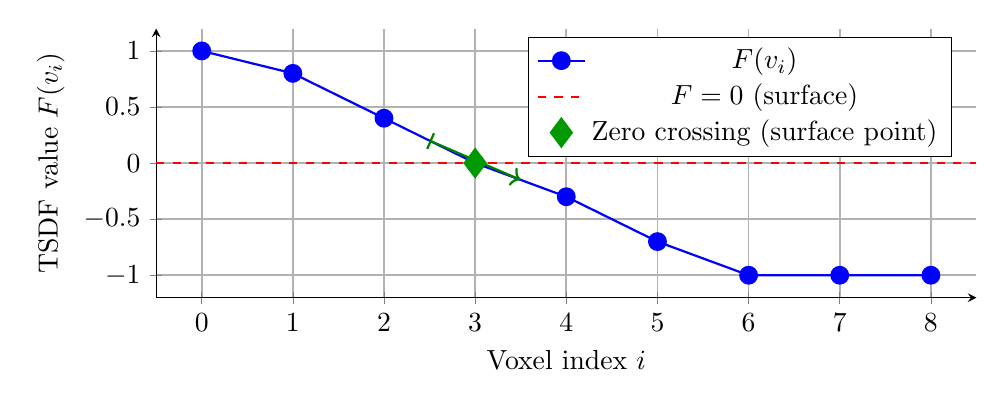
\begin{tikzpicture}
\begin{axis}[
    width=12cm, height=5cm,
    xlabel={Voxel index $i$},
    ylabel={TSDF value $F(v_i)$},
    xmin=-0.5, xmax=8.5,
    ymin=-1.2, ymax=1.2,
    xtick={0,1,2,3,4,5,6,7,8},
    ytick={-1,-0.5,0,0.5,1},
    grid=both,
    grid style={line width=0.3pt, draw=gray!30},
    major grid style={line width=0.6pt, draw=gray!60},
    axis lines=left,
    legend pos=north east
]
% TSDF values: positive outside, negative inside
\addplot[blue, thick, mark=*, mark size=3pt] coordinates {
    (0, 1.0) (1, 0.8) (2, 0.4) (3, 0.0) (4, -0.3) (5, -0.7) (6, -1.0) (7, -1.0) (8, -1.0)
};
\addlegendentry{$F(v_i)$}
% Zero line
\addplot[red, dashed, thick] coordinates {(-0.5, 0) (8.5, 0)};
\addlegendentry{$F=0$ (surface)}
% Highlight zero crossing
\addplot[green!60!black, thick, mark=diamond*, mark size=5pt, only marks] coordinates {(3, 0.0)};
\addlegendentry{Zero crossing (surface point)}
% Mark the sign change
\draw[|->, green!50!black, thick] (axis cs: 2.5, 0.2) -- (axis cs: 3.5, -0.15);
\node[green!50!black, font=\small] at (axis cs: 4.5, 0.4) {sign change};
\end{axis}
\end{tikzpicture}
\caption{1D TSDF cross-section. Positive values (blue, $i < 3$) indicate free space; negative values ($i > 3$) indicate occupied space. The zero crossing at $i \approx 3$ marks the surface. The bug extracted all voxels where $F \neq 0$ (nearly everything); the fix extracts only zero-crossing voxels.}
\label{fig:tsdf-1d}
\end{figure}

\subsection{2D TSDF Grid with Zero-Crossing Boundary}

Figure~\ref{fig:tsdf-2d} shows a 2D voxel grid with TSDF values and the zero-crossing boundary highlighted.

\begin{figure}[h!]
\centering
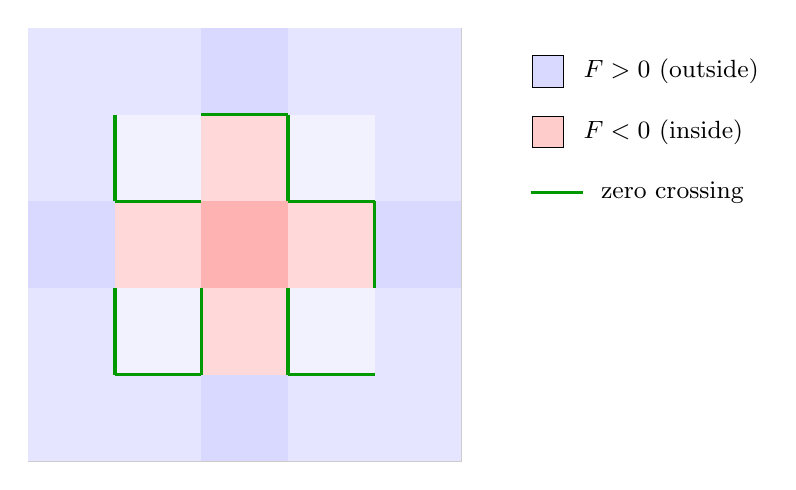
\begin{tikzpicture}[scale=1.1]
% Draw 5x5 grid
\foreach \i in {0,...,4} {
    \foreach \j in {0,...,4} {
        \draw[gray!40] (\i,\j) rectangle (\i+1,\j+1);
    }
}

% TSDF values: approximate circular surface at center (2.5,2.5), radius 1.5
% Positive = outside, negative = inside
% Row j=0 (bottom): all positive
\node[font=\tiny] at (0.5,0.5) {+1.0}; \fill[blue!10] (0,0) rectangle (1,1);
\node[font=\tiny] at (1.5,0.5) {+0.8}; \fill[blue!10] (1,0) rectangle (2,1);
\node[font=\tiny] at (2.5,0.5) {+0.5}; \fill[blue!15] (2,0) rectangle (3,1);
\node[font=\tiny] at (3.5,0.5) {+0.8}; \fill[blue!10] (3,0) rectangle (4,1);
\node[font=\tiny] at (4.5,0.5) {+1.0}; \fill[blue!10] (4,0) rectangle (5,1);
% Row j=1
\node[font=\tiny] at (0.5,1.5) {+0.8}; \fill[blue!10] (0,1) rectangle (1,2);
\node[font=\tiny] at (1.5,1.5) {+0.3}; \fill[blue!5] (1,1) rectangle (2,2);
\node[font=\tiny] at (2.5,1.5) {-0.2}; \fill[red!15] (2,1) rectangle (3,2);
\node[font=\tiny] at (3.5,1.5) {+0.3}; \fill[blue!5] (3,1) rectangle (4,2);
\node[font=\tiny] at (4.5,1.5) {+0.8}; \fill[blue!10] (4,1) rectangle (5,2);
% Row j=2
\node[font=\tiny] at (0.5,2.5) {+0.5}; \fill[blue!15] (0,2) rectangle (1,3);
\node[font=\tiny] at (1.5,2.5) {-0.2}; \fill[red!15] (1,2) rectangle (2,3);
\node[font=\tiny] at (2.5,2.5) {-0.9}; \fill[red!30] (2,2) rectangle (3,3);
\node[font=\tiny] at (3.5,2.5) {-0.2}; \fill[red!15] (3,2) rectangle (4,3);
\node[font=\tiny] at (4.5,2.5) {+0.5}; \fill[blue!15] (4,2) rectangle (5,3);
% Row j=3
\node[font=\tiny] at (0.5,3.5) {+0.8}; \fill[blue!10] (0,3) rectangle (1,4);
\node[font=\tiny] at (1.5,3.5) {+0.3}; \fill[blue!5] (1,3) rectangle (2,4);
\node[font=\tiny] at (2.5,3.5) {-0.2}; \fill[red!15] (2,3) rectangle (3,4);
\node[font=\tiny] at (3.5,3.5) {+0.3}; \fill[blue!5] (3,3) rectangle (4,4);
\node[font=\tiny] at (4.5,3.5) {+0.8}; \fill[blue!10] (4,3) rectangle (5,4);
% Row j=4 (top)
\node[font=\tiny] at (0.5,4.5) {+1.0}; \fill[blue!10] (0,4) rectangle (1,5);
\node[font=\tiny] at (1.5,4.5) {+0.8}; \fill[blue!10] (1,4) rectangle (2,5);
\node[font=\tiny] at (2.5,4.5) {+0.5}; \fill[blue!15] (2,4) rectangle (3,5);
\node[font=\tiny] at (3.5,4.5) {+0.8}; \fill[blue!10] (3,4) rectangle (4,5);
\node[font=\tiny] at (4.5,4.5) {+1.0}; \fill[blue!10] (4,4) rectangle (5,5);

% Highlight zero-crossing boundary edges in green
\draw[green!60!black, very thick] (1,1) -- (2,1); % between (1,1)=+0.3 and (2,1)=-0.2
\draw[green!60!black, very thick] (1,1) -- (1,2); % between (1,1)=+0.3 and (1,2)=-0.2
\draw[green!60!black, very thick] (2,1) -- (2,2); % vertical
\draw[green!60!black, very thick] (3,1) -- (3,2); % between (3,1)=+0.3 and (3,2)=-0.2 (via (2,2))
\draw[green!60!black, very thick] (3,1) -- (4,1); % horizontal
\draw[green!60!black, very thick] (1,3) -- (1,4);
\draw[green!60!black, very thick] (1,3) -- (2,3);
\draw[green!60!black, very thick] (2,4) -- (3,4);
\draw[green!60!black, very thick] (3,3) -- (4,3);
\draw[green!60!black, very thick] (3,3) -- (3,4);
\draw[green!60!black, very thick] (4,2) -- (4,3);

% Legend
\node[draw, fill=blue!15, minimum width=0.4cm, minimum height=0.4cm] at (6, 4.5) {};
\node[right, font=\small] at (6.3, 4.5) {$F > 0$ (outside)};
\node[draw, fill=red!20, minimum width=0.4cm, minimum height=0.4cm] at (6, 3.8) {};
\node[right, font=\small] at (6.3, 3.8) {$F < 0$ (inside)};
\draw[green!60!black, very thick] (5.8, 3.1) -- (6.4, 3.1);
\node[right, font=\small] at (6.5, 3.1) {zero crossing};

\end{tikzpicture}
\caption{2D TSDF voxel grid. Blue voxels have $F > 0$ (outside surface); red voxels have $F < 0$ (inside). Green edges mark zero-crossings --- the surface boundary. The correct \texttt{fetchPoints()} extracts only points near these green edges, not the entire grid.}
\label{fig:tsdf-2d}
\end{figure}

\section{Correctness of the Fix}

\begin{theorem}[Fix Correctness]
The zero-crossing condition $F(\mathbf{v}) \cdot F(\mathbf{v}') < 0$ for neighbor pairs $(\mathbf{v}, \mathbf{v}')$ correctly identifies all and only the voxel pairs that straddle the implicit surface $\{F = 0\}$, assuming $F$ is piecewise linear between voxels.
\end{theorem}

\begin{proof}
By the intermediate value theorem (IVT), a continuous function $f$ with $f(a) \cdot f(b) < 0$ must have a zero in $(a,b)$. For piecewise-linear $F$, the IVT applies between adjacent voxel centers. Conversely, if $F(\mathbf{v}) \cdot F(\mathbf{v}') > 0$, no zero exists in the segment (same sign throughout). Therefore the sign-change condition is both necessary and sufficient for a zero crossing.
\end{proof}

\section{References}

\begin{enumerate}
  \item Curless, B., Levoy, M. \textit{A Volumetric Method for Building Complex Models from Range Images}. SIGGRAPH, 1996.
  \item Newcombe, R.A., et al. \textit{KinectFusion: Real-Time Dense Surface Mapping and Tracking}. ISMAR, 2011.
  \item Lorensen, W.E., Cline, H.E. \textit{Marching Cubes: A High Resolution 3D Surface Construction Algorithm}. SIGGRAPH, 1987.
  \item Nießner, M., et al. \textit{Real-time 3D Reconstruction at Scale using Voxel Hashing}. ACM TOG, 2013.
  \item OpenCV 3D Module. \textit{hash\_tsdf.cpp}. OpenCV repository.
\end{enumerate}

\end{document}
